\chapter{Proposta}
\label{ch:proposta}

Este capítulo destina-se a explanar a proposta para o problema apresentado. De antemão são apresentadas as escolhas de arquitetura realizadas, referente aos tópicos levantados na Seção \ref{ch:fundamentos}, as justificativas a respeito de cada escolha são explanadas na Seção \ref{}. 

%
\section{Atores participantes}

Os atores que fazem parte da execução do protocolo são, primeiramente os clientes, que entram na rede em busca da escolha de um provedor que atenda aos seus padrões de preço e reputação para realizar a alocação de microsserviços. Seus poderes envolvem o pedido devidamente organizado de uma alocação para a rede, a confirmação de propostas de provedores, prolongação de requisições, convocações de votação para possíveis quebras de contrato e o voto em convocações de outros usuários contra o seu provedor. O segundo grupo de participantes são os provedores, que adentram a rede em busca de novos clientes. Seus poderes envolvem responder a pedidos de alocação com propostas para um ou mais microsserviços distintos e votar em convocações para outros provedores. O terceiro grupo de participantes são os agregadores, que possuem todos os poderes de cliente e provedor mesclados, salvaguardando as requisições de serviço que são puramente para \acp{IaaS} genéricos, não sendo relacionadas a um conjunto de microsserviços como é o caso das requisições dos clientes. 

\section{Definições iniciais da rede}
\label{sec:proposta:definicoes}

O modelo da rede de \textit{Blockchain} escolhido assemelha-se ao do \textit{Bitcoin}, ou seja, fundamentalmente baseada em transações e que utiliza as informações dessas para levantar a situação atual do usuário.
%
A rede proposta, entretanto, não tem seu fim em transações monetárias, assim não trata-se de uma criptomoeda em essência, porém utiliza certas características normalmente adotadas nelas em conjunto com propriedades destoantes que melhor refletem as necessidades do problema abordado.

%
A maioria das informações que transitam entre usuários e que consequentemente são escritas na cadeia se referem puramente a dados de definição e concretização de contratos, desenvolvidas para otimizar e facilitar o processo de contratação de infraestruturas, bem como para possível avaliação posterior.
%
Apenas uma pequena parcela do total de transações conterá movimentação de valores propriamente ditos e estes não servirão como moeda de troca mas sim como medidor da reputação dos participantes. Quanto maior for o montante desse valor possuído por um usuário - referidos a partir do presente momento como pontos de reputação - naturalmente melhor será sua reputação. Esse valor será obrigatoriamente público - característica que novamente destoa das criptomoedas apresentadas no Capítulo \ref{ch:fundamentos} - tanto para os participantes da rede quanto para indivíduos externos. Essa propriedade é definida dessa maneira para atender a um dos objetivos do protocolo que é auxiliar clientes na escolha de provedores de serviço, no qual a reputação é um fator importante. Partindo de tais fatos e complementando a definição da Seção \ref{subsec:blockchain:pub_priv}, a proposta trata-se de uma rede de consórcio, pois apenas um grupo aprovado de usuários pode operar sobre a cadeia, na qual a entrada está sujeita à apresentação de provas de identidade para provedores e agregadores, de modo a garantir a integridade dos processos que nela acontecem. A pesquisa e visualização dos dados na \textit{Blockchain} é pública, logo até usuários que não possuem nenhuma correlação com o sistema podem visualizar dados de transações e de reputação.

%
Na rede os usuários possuem endereços individuais, responsáveis por identificá-los em meio aos outros participantes e possuem também um endereço de grupo, que identifica qual é o tipo daquele usuário. A segunda característica é importante pois como grande parte das transações trata-se de publicação de informações, torna-se interessante que mais de um usuário possa referenciar certos tipos de transação para diversos fins apresentados nas Seções \ref{sec:proposta:fase_contratual} e \ref{sec:proposta:fase_auditoria}.

%
Da mesma forma que no mundo real, não é possível vender ou transferir reputação de uma pessoa ou organização para outra, tal característica também poderá ser observada na rede, portanto um usuário não pode deliberadamente criar uma transação para transferir pontos de reputação. Contudo, a movimentação de tais pontos de fato acontece, embora a parte majoritária das decisões a respeito dessas transferências não caibam ao usuário, mas sim ao protocolo em si e ao processamento distribuído, fato elucidado na Seção \ref{sec:cenario_execucao}. No que toca a execução distribuída no contexto de \textit{Blockchain}, uma grande personagem no processo é a carteira digital ou, de forma mais genérica, o cliente de acesso à rede. Na rede proposta a carteira terá um papel significativo pois além de ser responsável por administrar as chaves, gerar endereços e validar transações e blocos, ainda terá a responsabilidade de julgar quando houve quebra de contrato, também administrando módulos remotos encarregados do processo de monitoração, conceito retomado na Seção \ref{sec:cenario_execucao}.

%
Ao retomar as formas de consenso exploradas na Seção \ref{subsec:blockchain:consenso} conclui-se que o uso de \ac{PoW} convencional não é adequado para tal cenário, porque como agregadores e especialmente provedores podem alocar poderes computacionais elevados para mineração, quando comparados aos usuários, a parte majoritária das minerações seriam de autoria de provedores e agregadores, com apenas aparições esparsas de blocos criados por usuários comuns. Um ambiente como esse, além de injusto com usuários menos favorecidos computacionalmente, implica em uma grande carga de responsabilidade e confiança em um grupo relativamente pequeno de usuários. Esses, mesmo possuindo um histórico possivelmente idôneo também podem vir a praticar ações fraudulentas, de forma que não é possível garantir que manterão o comportamento correto no decorrer da criação dos blocos futuros.

\section{Cenário de execução}
\label{sec:cenario_execucao}

Essa seção tem por objetivo elencar o cenário de execução principal da proposta, assim como características iniciais relativas à estrutura das trocas de mensagens, ordem das mesmas e a relação dos atores com a cadeia e uns para com os outros.

%
O cerne do protocolo, como apontado na Seção \ref{ch:intro} reside na elaboração e verificação de contratos. Para o primeiro passo utiliza-se a cadeia de blocos como forma de comunicação assíncrona e meio de sedimentação das negociações ao longo do tempo. Para a segunda parte, decorrentes de suspeitas de violações de contrato, são convocadas votações a respeito da ocorrência ou não de quebra. Estas são respaldadas por dados de monitoração obtidos por usuários e agregadores que possuem algum tipo de relação contratual de \ac{IaaS} para com o agregador ou provedor sendo acusado, mas também por provedores e agregadores que embora não possuam contratos monitoram seus concorrentes secretamente.

%
As escritas na cadeia - referidas também como transações - quando não assumem o caráter de transferência de pontos de reputação podem ser entendidas como uma publicação e sedimentação de informações, sendo que essas podem ser referenciadas pelos participantes para a realização de novos conjuntos de transações, que resultam na sedimentação de mais informações e assim por diante. Todas essas informações escritas na rede relacionam-se de alguma forma com a elaboração dos contratos e servem basicamente como veículo de comunicação e forma de estabelecer e armazenar os contratos em si. 
%
As transações voltadas para a transferência de pontos de reputação acontecem no estabelecimento de um novo contrato, pois o agregador ou provedor que prestará o serviço ou parte dele tem sua reputação verificada pelo usuário contratante e após a confirmação do contrato entende-se que o usuário confia naquele prestador de serviço. Assim, olhando de forma pragmática, a reputação de um provedor ou agregador é dada pela quantidade de clientes satisfeitos que eles possuem e assume-se que um cliente que acaba de iniciar um contrato está satisfeito, tendo em vista que perante análise inicial as condições do contrato são de seu interesse e não foram violadas.
%
De forma análoga, um provedor ou agregador perderá pontos de reputação quando for declarado culpado de quebra de contrato mediante uma acusação relacionada. Pontos de reputação podem ainda ficar em custódia temporária durante processos de votação, onde é possível que participantes terceiros ganhem ou percam reputação de acordo com a contribuição de dados assertivos ou não, discussão que é retomada na Seção \ref{sec:proposta:fase_auditoria}. 
%
Relativamente, a monitoração entre provedores e agregadores responsável por gerar os dados para votações, não depende necessariamente de nenhum contrato, ou seja, assim que um novo provedor entra na rede ele pode começar a ser monitorado e da mesma forma monitorar seus concorrentes.

%
Para auxiliar a formação do cenário de execução hipotético nas Seções \ref{sec:proposta:fase_contratual} e \ref{sec:proposta:fase_auditoria} é utilizada a figura \ref{fig:cenario_execucao} que trata todas as nuances do processo, envolvendo desde a requisição de serviço até o veredito de violação.

\begin{figure}[h!]
\caption{Cenário de execução completo}
\centering
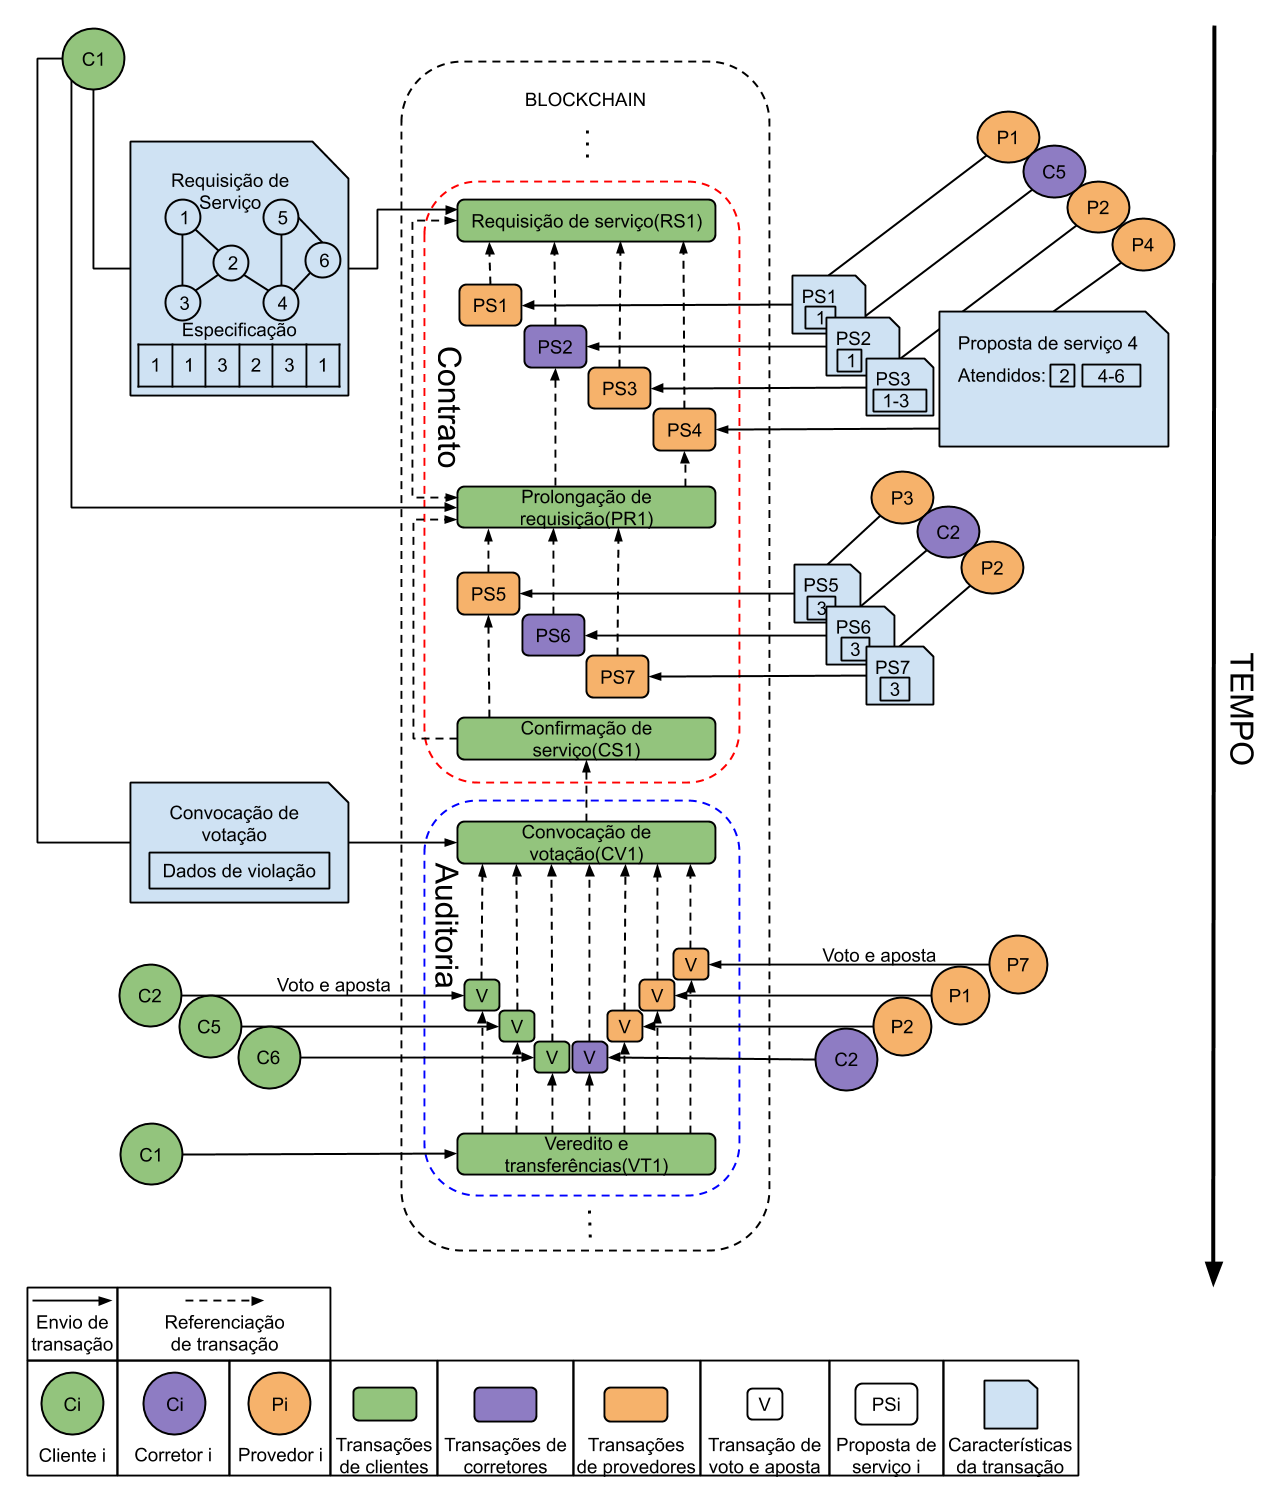
\includegraphics[width=0.96\textwidth]{imagens/cenario_execucao.png}
\begin{center}
        Fonte: Autor
\end{center}
\label{fig:cenario_execucao}
\end{figure}


Assim, clientes envolvidos no processo são representados por círculos verdes e por uma legenda contendo a letra maiúscula C, bem como um índice numérico referente ao cliente em questão. O mesmo vale para provedores e agregadores, que além de serem reconhecidos pelos índices individuais, são representados por círculos laranjas e pela letra P, no caso dos provedores e círculos roxos e pela letra A, no caso dos agregadores. A cadeia de blocos é representada por um retângulo tracejado e referenciações para transações passadas são identificadas através de flechas tracejadas em direção à transação pai. Envios de transações para a rede por parte dos atores são representados por flechas contínuas que iniciam no ator e terminam dentro da \textit{Blockchain}. Detalhes importantes das transações enviadas são mostrados através de retângulos azuis no meio das flechas de envio. Transações de autoria de usuários na cadeia são coloridas de acordo com a cor referente ao tipo do mesmo. Outras Informações específicas a respeito da estrutura das transações e funcionamento de baixo nível do sistema serão explicadas na Seção \ref{}.

\section{Fase contratual}
\label{sec:proposta:fase_contratual}

A fase contratual representa o início de um ciclo completo do protocolo e compreende todo o processo relativo ao estabelecimento de um contrato e as negociações realizadas para tal. Essa fase é representada na Figura \ref{fig:cenario_execucao} por um retângulo tracejado vermelho com a legenda "Contrato".


\subsection{Requisições de serviço}
\label{subsec:proposta:contratual:rs}
%
Os contratos na rede proposta devem ser atômicos, assim não é possível fechar um contrato sem que todos os microsserviços elencados pelo cliente sejam devidamente supridos pela infraestrutura de algum provedor ou agregador. Após a entrada de um usuário na rede este já está apto a estabelecer contratos com provedores, o primeiro passo para realizar esse processo é a escrita de uma nova transação, que representa uma requisição de serviço. Essa requisição de serviço descrevem um conjunto de microsserviços que, como pode ser observado na figura \ref{fig:cenario_execucao}, são organizados em um grafo não direcionado, de forma que os nós representam os microsserviços em si e as arestas os enlaces necessários para que a comunicação seja realizada corretamente. Junto ao grafo encontra-se um vetor com tamanho igual à quantidade de microsserviços, cujo valor de cada célula $i$ representa a infraestrutura requerida para o microsserviço $i$. Por fim, há uma quantidade finita de requisições de serviço abertas que um usuário pode ter em um determinado momento, de modo que quando esse limite é atingido é necessário fechar contratos - se todos os microsserviços foram atendidos com infraestruturas correspondentes - ou finalizá-las para que a criação de novas requisições seja liberada.

\subsection{Definições de infraestrutura}
\label{subsec:proposta:contratual:di}
%
Diferentes microsserviços de uma mesma requisição podem ter necessidades diferentes de infraestrutura e portanto as transações de \ac{RS} devem referenciar outras transações chamadas \ac{DI}, que podem ou não ser escritas pelo usuário que faz a requisição. Na rede, qualquer participante pode escrever um número finito de transações de \ac{DI} e estas podem ser referenciadas por qualquer outro usuário que deseja fazer uma requisição. Assim sendo, provedores podem publicar definições padrão que costumam oferecer, como se fossem planos predefinidos de serviço, enquanto usuários podem criar novas definições para microsserviços com necessidades específicas que podem, eventualmente, servir para outros usuários em condições semelhantes. Atualizações nas definições podem ser feitas pelos criadores em caso da necessidade de adaptação de infraestruturas para novos contratos, sendo representadas por uma nova \ac{DI} que referencia a anterior. \acp{DI} apenas podem ser atualizadas caso já exista algum contrato firmado que as referenciem, para evitar o surgimento de definições órfãs ou o superpovoamento de definições pelos usuários. Portanto, usuários podem ter até $n$ definições existentes sem referenciação e nada impede o criador ou outros clientes de referenciar versões passadas de uma \ac{DI}.

%
O objetivo dessa escolha de arquitetura é primeiramente reduzir a duplicação de informação, uma vez que muitos clientes podem querer utilizar arquiteturas idênticas, cujas diferentes requisições de serviço não precisam reter as informações consigo, mas apenas referenciá-las. Consequentemente, as dificuldades de escalabilidade da rede se tornam mais brandas, devido ao menor volume de dados que é precisa armazenar em todos os dispositivos conectados. Esse tipo de abordagem leva à consequente formação de uma "biblioteca" pública de definições de infraestrutura, na qual usuários publicam informações e utilizam as de terceiros.

%
\subsection{Propostas de serviço}
\label{subsec:proposta:contratual:PS}

Após a escrita de uma \ac{RS} na cadeia, propostas de serviço podem ser enviadas para suprir tal demanda. \acp{RS} são escritas de modo que a saída da transação seja travada não para o endereço de um usuário, mas sim para endereços do grupo de agregadores e para o grupo de provedores. Esses podem referenciar a requisição em questão criando novas transações chamadas \ac{PS}, que contém uma oferta da infraestrutura desejada para um ou mais microsserviços. Uma informação importante contida em tal forma de transação é o preço que o provedor se dispõem a realizar o serviço descrito na proposta, uma vez que grande parte das informações a respeito da alocação em si já foram definidas na \ac{DI} referenciada pela requisição.

\subsection{Prolongação de requisição}
\label{subsec:proposta:contratual:pr}
%
Um cliente, após abrir uma requisição, pode esperar por tempo indeterminado propostas de serviço até encontrar as que mais se adéquem às suas preferências. Ocasionalmente, o aparecimento de novas propostas para uma requisição cessa, decorrente do envelhecimento da transação em questão na cadeia, que acarreta em baixa visibilidade para outros provedores. Outro possível cenário trata-se do cliente se interessar por propostas que contemplam uma parcela dos microsserviços, mas não por aquelas que contemplam outra, da mesma forma que a requisição pode não receber propostas suficientes para abranger os microsserviços em completude. Na ocorrência de tais casos, o usuário pode criar uma \ac{PR} que serve para explicitar quais das propostas feitas até o momento foram escolhidas para a requisição, sendo indicadas através da referenciação das transações das \acp{PS}. Após a criação dessa transação, o efeito gerado na rede é o reavivamento da requisição, que acontece devido a transmissão da \ac{PR} como uma nova transação, atraindo o olhar de provedores e agregadores. Na prolongação deve ser registrado, além das propostas aceitas, quais microsserviços não foram atendidos, de modo a agilizar o processo posterior de verificação dessas transações, para que não seja necessário vasculhar a cadeia toda para encontrar a requisição e obter tais dados.
%
Novas \ac{PS} podem então ser feitas por parte dos prestadores de serviço, agora referenciando não a requisição original, mas sim a prolongação de requisição relacionada, buscando assim finalizar o processo de escolha dos serviços. A quantidade de \ac{PR} que uma requisição pode ter é limitada, pois pode ocorrer de que certos microsserviços apenas não sejam mercadologicamente viáveis para o atendimento dos prestadores. Em face de tal ocorrido, a única alternativa é recomeçar o processo criando uma requisição em que as características dos microsserviços não atendidos sejam modificadas. Entretanto, presume-se que o aparecimento do referido cenário é esparso e que a maioria das requisições são completamente atendidas.

\subsection{Confirmação de serviço}
\label{subsec:proposta:contratual:di}

O último processo da fase contratual é a \ac{CS}, nela o usuário cria uma transação que deve referenciar as propostas de serviço restantes da última \ac{PR} ou, no caso de não haver nenhuma, a \ac{RS} original. Essa transação é de suma importância pois é responsável por selar o contrato de \ac{IaaS} com todos os provedores e suas \acp{PS} selecionadas no processo até então. A partir da existência de uma \ac{CS} na cadeia, nenhuma nova proposta de serviço que referencia a requisição ou prolongações dessa \ac{CS} passa no processo de validação por qualquer nó. A alocação das infraestruturas oficializadas pelo protocolo não é regida nem supervisionada por ele, porém acredita-se que nenhum dos atores envolvidos tem motivos para não realizá-la no mundo real, pois o prestador do serviço quer vender o produto(\textit{i.e.} obter lucro) e o cliente quer sua aplicação funcionando no mercado. Mesmo em casos esdrúxulos nos quais por algum motivo a alocação não ocorra de verdade, esse contrato não afeta o futuro da rede, porque o voto em acusações contra qualquer um dos provedores envolvidos depende das provas criptográficas de monitoração, que invariavelmente não existirão sem a alocação física. Após a criação e validação de uma confirmação de serviço, já é possível que a fase de auditoria seja iniciada.

\section{Fase de auditoria}
\label{sec:proposta:fase_auditoria}

A a fase de auditoria ocorre quando um usuário detecta que seu contrato foi violado pelo provedor e medidas para auditoria da ocorrência de quebra ou não, são então tomadas pela rede. Essa fase é representada por um retângulo tracejado azul com a legenda "Auditoria". Essa fase baseia-se em dois pilares fundamentais, sendo o primeiro o contrato estabelecido e os dados do mesmo existentes na \textit{Blockchain} e o segundo um conjunto de dados relativos à execução da alocação, coletados por um módulo de monitoração auxiliar da carteira. Usuários clientes monitoram exclusivamente provedores com os quais possuem algum contrato firmado, ao passo que usuários provedores e agregadores podem - e é de seus interesses - monitorar outros usuários desses mesmos grupos. A inter-monitoração de prestadores de serviço ocorre de maneira paralela à cadeia, assim dados recolhidos são mantidos localmente pelo realizador do processo e fornecidos aos outros usuários apenas como comprovação de voto no momento apropriado. Esses dados, embora possuam um dono teórico e sejam eventualmente compartilhados, não devem ser interpretáveis por nenhum agente que não a carteira digital em si de cada usuário. Dessa forma, mesmo o agente externo que possui controle sobre a carteira não consegue entender os dados que produz ou recebe, sendo que a coerência empírica desses apenas existe no contexto de execução da carteira, que é alheio ao usuário.

\subsection{Convocação de votação}
\label{sec:proposta:auditoria:cv}

